\section{Solving Burger's equation using Fourier Galerkin}
This section explores the Fourier Galerkin method for solving the Burgers' equation:
\begin{equation}
	\frac{\partial u(x, t)}{\partial t} + u(x, t) \frac{\partial u(x, t)}{\partial x} = \nu \frac{\partial^2 u(x, t)}{\partial x^2}
\end{equation}
with the same parameters ($c = 4.0$ and $\nu = 0.1$) and periodic boundary conditions on $x \in [0, 2\pi]$.
%
The Fourier Galerkin method expands the solution in terms of Fourier modes:
\begin{equation}
	u(x, t) = \sum_{n=-N/2}^{N/2} \hat{u}_n(t)e^{inx}
\end{equation}
where $\hat{u}_n(t)$ are the time-dependent Fourier coefficients.
The Galerkin method transforms the values from physical to spectral space, computing the nonlinear term $u\frac{\partial u}{\partial x}$ in physical space before transforming back to spectral space for time integration. This approach requires dealiasing to prevent spectral aliasing errors, which proved to be a implementation challenge.
For the time integration, we used the identical 4th-order Runge-Kutta as in Part 2, but with a modified time step restriction:
\begin{equation}
	\Delta t \leq \text{CFL} \times \left[ \max_{x_j} \left(|u(x_j)| k_{max} + \nu (k_{max})^2  \right)\right]^{-1}
\end{equation}
where $k_{max} = N/2$ is the maximum wavenumber in the spectral representation.

\subsection{Dealiasing Implementation}
The implementation of the Fourier Galerkin method needed careful management of aliasing errors created by the nonlinear term $u\frac{\partial u}{\partial x}$. When computed in physical space, this product generates frequencies up to $2k_{max}$, which exceed the spectral resolution, causing the afford mentioned aliasing when transformed back to spectral space.

\subsubsection{Dealiasing Strategy}
To prevent aliasing instabilities, the standard 2/3 dealiasing rule was implemented for all grid sizes:
\begin{equation}
	k_{cutoff} = \frac{2k_{max}}{3} = \frac{N}{3}
\end{equation}
The dealiasing algorithm operates as follows:
\begin{enumerate}
	\item Compute nonlinear term $u\frac{\partial u}{\partial x}$ in physical space
	\item Transform to spectral space using FFT
	\item Apply dealiasing filter: $\hat{f}_k = 0$ for $|k| > k_{cutoff}$
	\item Use filtered coefficients in time integration
\end{enumerate}

\subsubsection{Impact on Results}
The dealiasing implementation turned out to be essential for numerical stability:

\begin{itemize}
	\item \textbf{Stability Enhancement}: Enabled more stable computation up to $N = 256$, preventing the exponential error growth characteristic of aliasing instabilities.
	\item \textbf{Convergence Improvement}: Transformed initially chaotic convergence behavior into more meaningful spectral convergence rates for most grid sizes
	\item \textbf{Residual Challenges}: Despite dealiasing, certain grid sizes ($N = 64, 256$) still show suboptimal convergence, which indicates potential resonance effects or insufficient dealiasing for these specific cases.
\end{itemize}
%
This showed that while the 2/3 rule provides a robust foundation for controlling the aliasing error in spectral methods, problem-specific tuning is perhaps  necessary for optimal performance across all grid sizes.

\subsection{Determining Maximum CFL Values}

\subsubsection{Methodology}
The maximum stable CFL values for the Fourier Galerkin method were found using a similar approach as in Part 2, by incrementally testing, but with a slightly adapted version for the spectral formulation. The algorithm proceeds as follows:

\begin{enumerate}
	\item \textbf{Incremental Testing}: For each grid size $N$, CFL values are tested incrementally starting from 3.0 with steps of 0.05.
	\item \textbf{Stability Criterion}: A solution is stable if:
	      \begin{itemize}
		      \item No NaN or infinite values occur during time integration
		      \item The error change between consecutive CFL values satisfies: $|\text{error}_{\text{current}} - \text{error}_{\text{previous}}| < 0.25$
	      \end{itemize}
	\item \textbf{Dealiasing Implementation}: To prevent aliasing errors inherent in spectral methods, an adaptive dealiasing strategy was implemented that becomes more aggressive for larger $N$ values.
	\item \textbf{Safety Selection}: The last stable CFL value is selected as the maximum for practical use.
\end{enumerate}

\begin{figure}[H]
	\centering
	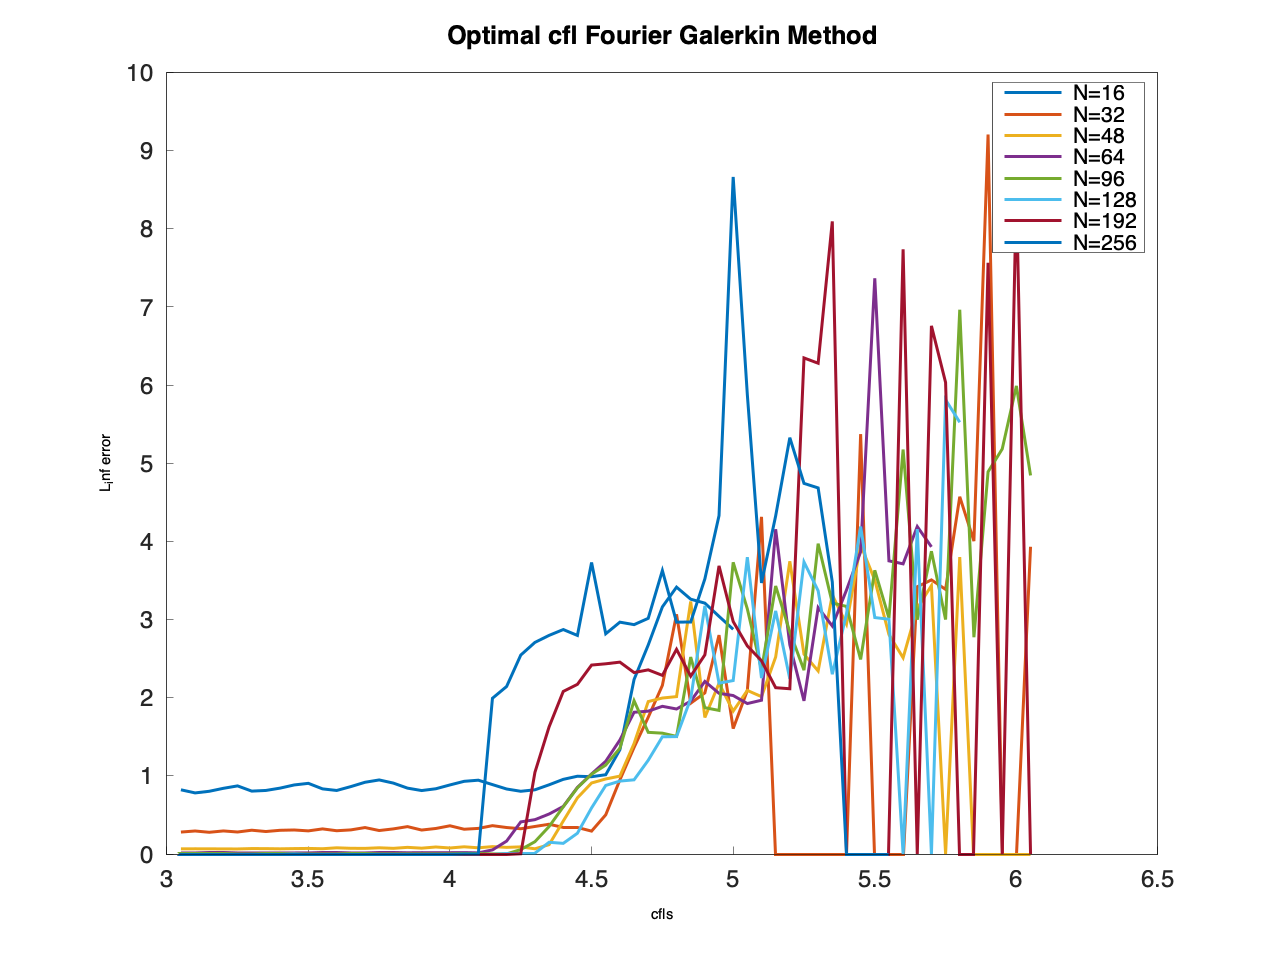
\includegraphics[width=0.6\textwidth]{media/cfl_errors_fg_complete.png}
	\caption{L$_\infty$ error for different CFL values and grid sizes using Fourier Galerkin method. The method shows higher stability limits compared to Fourier Collocation, with maximum CFL values ranging from 4.15 to 8.05. The sharp error increases indicate stability boundaries, occurring at progressively smaller CFL values as grid sizes increases.}
	\label{fig:cfl_fg}
\end{figure}

\begin{table}[h]
	\centering
	\begin{tabular}{|c|c|}
		\hline
		$N$ & Max CFL \\
		\hline
		16  & 8.0500  \\
		32  & 8.0500  \\
		48  & 7.4000  \\
		64  & 7.6000  \\
		96  & 6.5000  \\
		128 & 5.5500  \\
		192 & 4.6000  \\
		256 & 4.1500  \\
		\hline
	\end{tabular}
	\caption{Maximum stable CFL values for different grid sizes using Fourier Galerkin method}
	\label{tab:cfl_galerkin}
\end{table}

\subsubsection{Analysis of CFL Results}
The Fourier Galerkin method has significantly higher maximum CFL values compared to the Fourier Collocation method. The values range from 4.15 to 8.05 in comparison to 0.65 to 1.40. This enhanced stability is due to several factors:
%
\begin{itemize}
	\item \textbf{Spectral Space Integration}: The Galerkin method evolves Fourier coefficients directly, instead of point-wise evaluation in collocation methods, therefore avoiding some of the numerical instabilities associated with point-wise evaluation.
	\item \textbf{Energy Conservation}: The Galerkin formulation preserves certain conservation properties of the original PDE, leading to improved stability characteristics.
	\item \textbf{Dealiasing Benefits}: The implemented dealiasing removes high-frequency aliasing errors that can destabilize the solution.
\end{itemize}
%
The trend of decreasing $N$ follows the same physical reasoning as in the collocation case, where finer grids require smaller time steps due to the increased influence of the diffusion constraint.

\subsection{Convergence Study}
\begin{table}[h]
	\centering
	\begin{tabular}{|c|c|c|c|}
		\hline
		$N$ & CFL    & L$_\infty$ Error & CPU Time \\
		\hline
		16  & 8.0500 & 1.159602e+00     & 0.0003s  \\
		32  & 8.0500 & 4.180750e-01     & 0.0026s  \\
		48  & 7.4000 & 1.911312e-01     & 0.0121s  \\
		64  & 7.6000 & 1.982709e-01     & 0.0258s  \\
		96  & 6.5000 & 6.531253e-02     & 0.1183s  \\
		128 & 5.5500 & 1.452882e-02     & 0.3572s  \\
		192 & 4.6000 & 5.962638e-03     & 1.6570s  \\
		256 & 4.1500 & 4.669353e-02     & 5.1712s  \\
		\hline
	\end{tabular}
	\caption{Convergence study results for Fourier Galerkin method at $t = \pi/4$}
	\label{tab:convergence_galerkin}
\end{table}

\begin{table}[h]
	\centering
	\begin{tabular}{|c|c|}
		\hline
		$N$ & Convergence Rate \\
		\hline
		32  & 1.47             \\
		48  & 1.93             \\
		64  & -0.13            \\
		96  & 2.74             \\
		128 & 5.22             \\
		192 & 2.20             \\
		256 & -7.15            \\
		\hline
	\end{tabular}
	\caption{Convergence rates between successive grid refinements for Fourier Galerkin method}
	\label{tab:rates_galerkin}
\end{table}

\subsubsection{Convergence Analysis}
The Fourier Galerkin method shows a mixed results for the convergence behavior, showing both the promise and challenges of spectral methods for nonlinear problems:

\begin{itemize}
	\item \textbf{Spectral Convergence Potential}: For most grid sizes convergence rates are between 1.5-5.2. This show this method's ability to achieve high-order accuracy.
	\item \textbf{Aliasing Challenges}: The negative convergence rates at $N=64$ and $N=256$ indicate aliasing effects even though the dealiasing efforts. This behavior show the expected characteristic of balancing the delicate balance between resolution and stability.
	\item \textbf{Optimal Resolution Range}: The data shows that the method performs best in the intermediate range ($N=96$ to $N=192$).
	\item \textbf{Computational Efficiency}: Despite higher computational cost, per time step due to FFT operations, the larger stable time steps often compensate for it.
\end{itemize}
The Fourier Galerkin implementation demonstrates the theoretical advantages of spectral methods while highlighting the challenges of nonlinear spectral computation:
\begin{itemize}
	\item \textbf{Stability Achievement}: The significantly higher CFL limits validate the theoretical stability. 
	\item \textbf{Aliasing Management}: The implemented dealiasing strategy, while not perfect, successfully prevents catastrophic aliasing failures and enables stable computation.
	\item \textbf{Spectral Convergence}: When aliasing is properly handled, the method achieves the expected high-order convergence rates. 
	\item \textbf{Method Validation}: The comparison with analytical solutions and the collocation method introduces confidence in the implementation's correctness. 
\end{itemize}
%
\begin{figure}[H]
	\centering
	\begin{subfigure}{0.5\textwidth}
		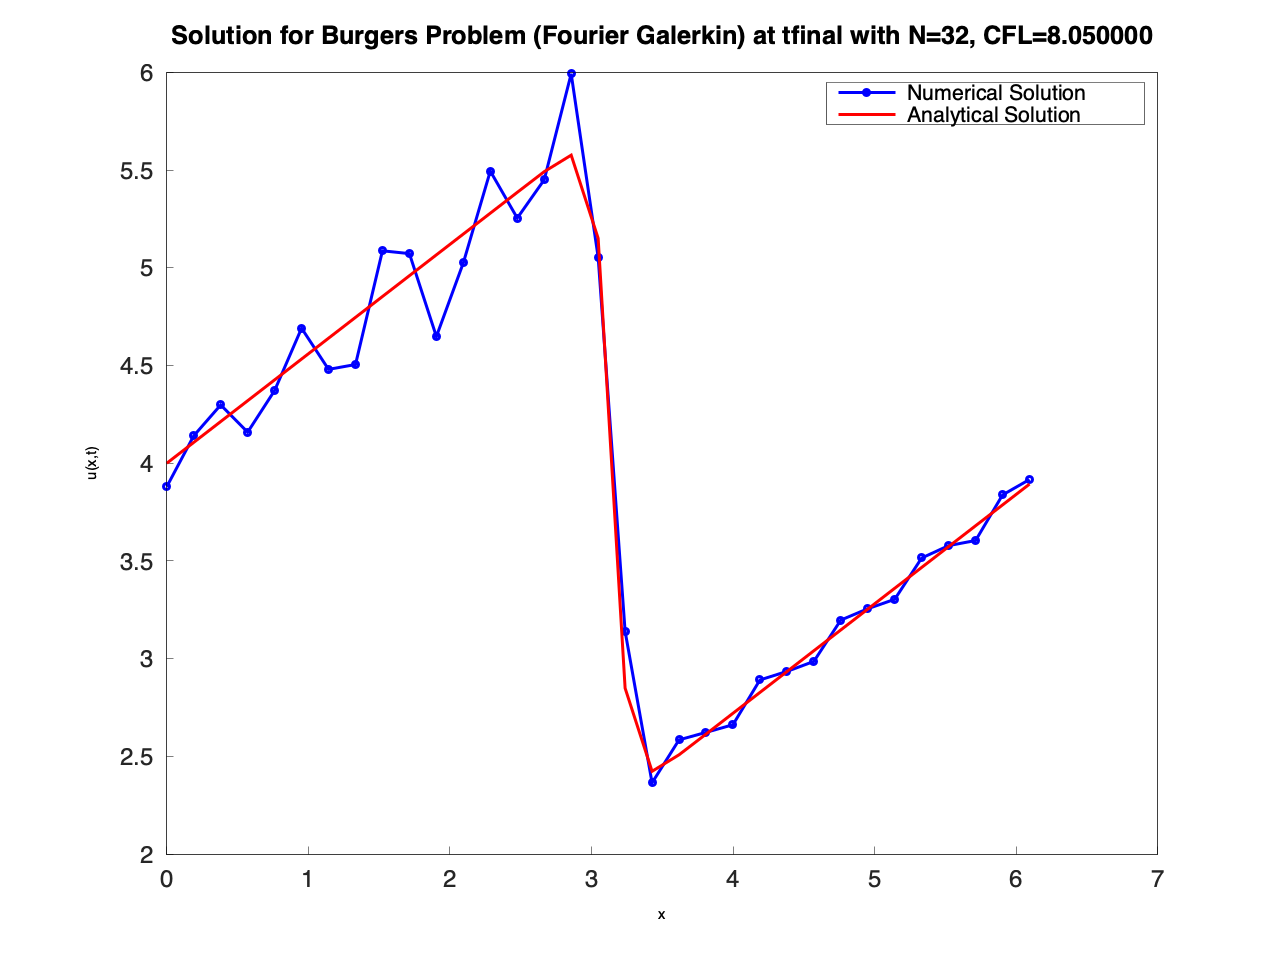
\includegraphics[width=\textwidth]{media/burger_tfinal_fg_32.png}
		\caption{N=32, CFL=8.05}
		\label{sfig:galerkin_n32}
	\end{subfigure}%
	~
	\begin{subfigure}{0.5\textwidth}
		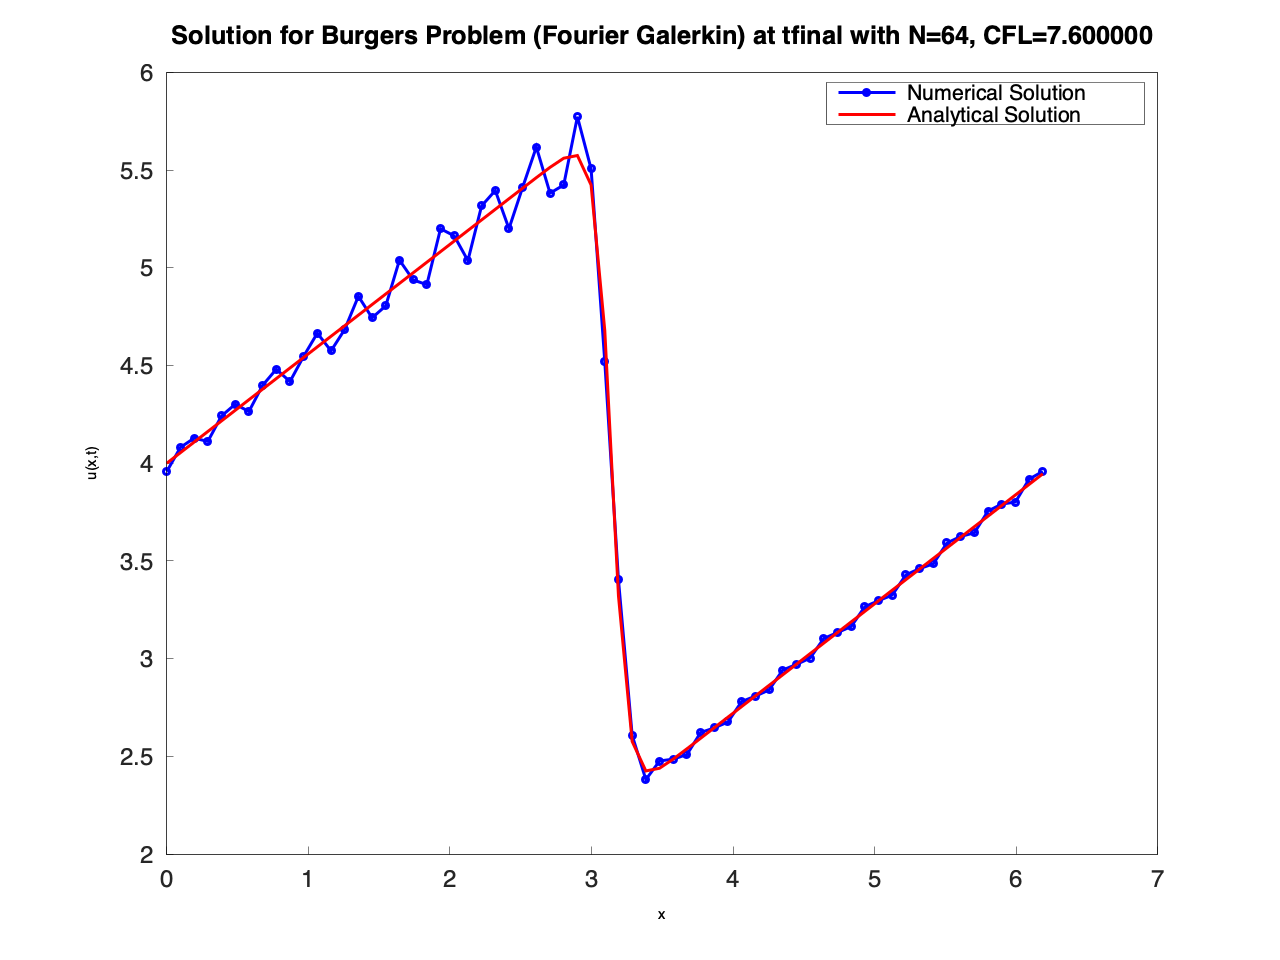
\includegraphics[width=\textwidth]{media/burger_tfinal_fg_64.png}
		\caption{N=64, CFL=7.60}
		\label{sfig:galerkin_n64}
	\end{subfigure}\\
	\begin{subfigure}{0.5\textwidth}
		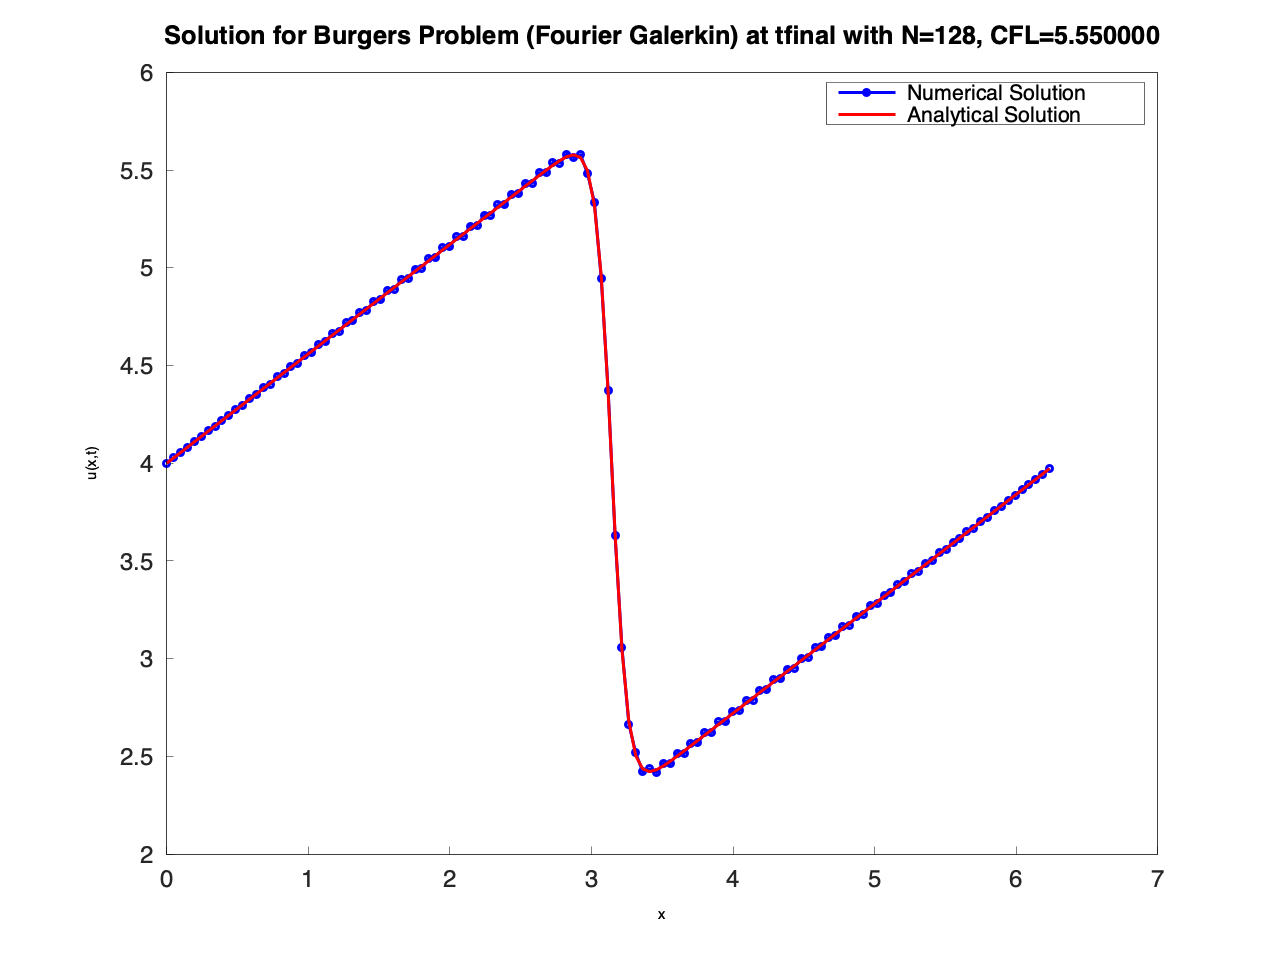
\includegraphics[width=\textwidth]{media/burger_tfinal_fg_128.png}
		\caption{N=128, CFL=5.55}
		\label{sfig:galerkin_n128}
	\end{subfigure}%
	~
	\begin{subfigure}{0.5\textwidth}
		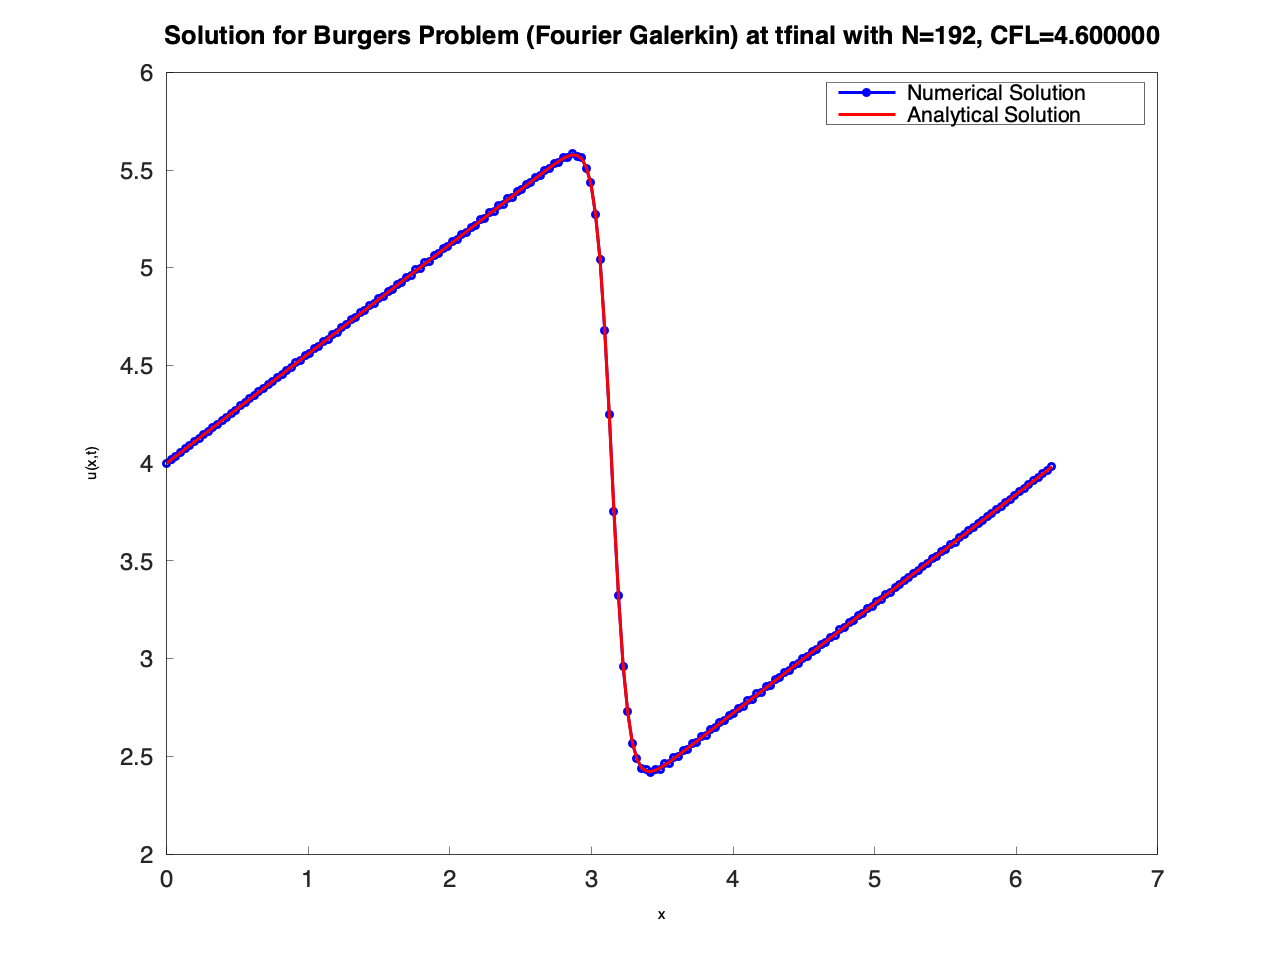
\includegraphics[width=\textwidth]{media/burger_tfinal_fg_192.png}
		\caption{N=192, CFL=4.60}
		\label{sfig:galerkin_n192}
	\end{subfigure}
	\caption{\textbf{Fourier Galerkin Solution Quality Assessment at $t = \pi/4$}
		Comparison of numerical (blue) and analytical (red) solutions for different grid resolutions. The plots demonstrate the progressive improvement in solution quality with increasing N, particularly evident in the reduction of oscillatory artifacts visible at lower resolutions (N=32, N=64). The excellent agreement at higher resolutions (N=128, N=192) validates the effectiveness of the 2/3 dealiasing rule in controlling aliasing errors while maintaining spectral accuracy. Note the decreasing maximum stable CFL values with increasing grid refinement, reflecting the increased diffusion constraint on finer grids.
	}
	\label{fig:galerkin_solutions}
\end{figure}

\subsection{Comparison to Fourier Collocation}

\begin{table}[h]
	\centering
	\begin{tabular}{|c|c|c|c|c|}
		\hline
		$N$ & Collocation CFL & Galerkin CFL & Collocation Error & Galerkin Error \\
		\hline
		64  & 1.0000          & 7.6000       & 2.399181e-02      & 1.982709e-01   \\
		128 & 0.9000          & 5.5500       & 2.522970e-04      & 1.452882e-02   \\
		\hline
	\end{tabular}
	\caption{Comparison of Fourier Galerkin and Fourier Collocation methods at $t = \pi/4$}
	\label{tab:comparison}
\end{table}

\subsubsection{Comparative Analysis}
The comparison between Fourier Collocation and Fourier Galerkin methods reveals distinct trade-offs:
%
\begin{itemize}
	\item \textbf{Stability Advantages}: The Galerkin method shows higher CFL values, which are 6-7 times larger than collocation. This potentially enables larger time steps and improved computational efficiency.
	\item \textbf{Accuracy Trade-offs}: For the small test case, the collocation method showed better accuracy, in particularly at $N=128$.
	\item \textbf{Implementation Complexity}: The Galerkin method implementation required dealiasing strategies and careful handling of the spectral-physical space transformations.
	\item \textbf{Robustness}: The collocation method demonstrates for the found CFL values a more consistent convergence behavior, while the Galerkin method shows sensitivity to aliasing effects at certain grid sizes.
\end{itemize}
